\chapter{State of the art}
\label{ch:marco}

\section{Related works}

The use of deep learning in agriculture has a great pontential in a variety of applications such as soil mapping, crop type classification, crop monitoring, pest detection and management, among others \cite{Kamilaris}. Most of the work related to the detection of diseases and pests in tomato make use of deep learning techniques, and specifically the supervised learning algorithms. In \cite{Fuentes2017_2} a proposal that makes use of CNN classifiers and object detectors like Faster R-CNN, Region-based Fully Convolutional Network or Single Shot Multibox Detector for the disease detections in tomato in South Korea. One of the problems that this project faced was the false positives in the classification. In \cite{Fuentes2018} a filter is proposed to reduce this issue.

In \cite{AsimeniaDimokranitou2017} the use of an adversarial autoencoder for the event detection in applications such as public security, health monitoring or intrusion detection. This corresponds to an unsupervised generative method just able to replicate regular data. This method has the advantage that the network is able to learn the main features that represent normal data.

In \cite{Baur2019} a new architecture proposal is presented to combine the variational autoencoder (VAE) and the generative adversarial networks, for the detection of anomalies in MR brain images. This new architecture is compared with other approaches like general VAE, spatial VAE, and AnoGAN. The authors claim that their VAEGAN architecture outperforms the other architectures.

\section{Methods}

\subsection{Deep Feedforward Networks}

The Deep Feedforward Networks, also known as multilayer perceptrons (MLPs), is the simplest structure  of artifitial neural network. The problem that this kind of network tackles is the approximation of some function \begin{math} f^{*}\end{math}. As mentioned in \cite{goodfellow_bengio_courville_2017}, a common example is in the implementation of a classifier where \begin{math} y = f^{*}(x)\end{math} maps the input \begin{math} x \end{math} to some category represented in \begin{math} y \end{math}. In order to achieve that, the feedforward networks defines a mapping of the form \begin{math} y = f(x, \theta)\end{math}, and during the training, this network adjusts the set of parameters \begin{math} \theta \end{math} that best approximate the function.

These networks are typically composed of many different functions, which represent the layers of the network. For example, we could have four layers that are connected in cascade, in the form \begin{math} f(x) = f_{(4)}(f_{(3)}(f_{(2)}(f_{(1)}(x)))) \end{math}. The length of these chains of functions can be seen as the depth of the network, where \begin{math} f_{(1)} \end{math} is the first layer, also known as the input layer, and \begin{math} f_{(4)} \end{math} is the last layer or the output layer. Between the first and the output layers are the hidden layers. During training, generally the output values corresponding to some input are explicited provided, but it is not specified what values the hidden layers should have. The learning algorithm decides how to use those hidden layers to generate the desired output.

\subsection{Convolutional Neural Networks}

The convolutional neural networks (CNN) \cite{Lecun1999} are an extension of the deep feedforward networks, that are specialized in the processing of grid-like data. As its name suggests, this kind of network makes use of the mathematical operation called convolution. The convolution is an operation on two functions of a real-valued argument and is defined as follows:

\begin{equation}
 s(x,y)=\sum_{u} \sum_{v} x(u,v) w(x-u,y-v)
\end{equation}

In terms of CNN, the first argument of the convolution (\begin{math} x(u,v) \end{math}) is referred as the input and the second argument (\begin{math} w(x-u,y-v) \end{math}) as the kernel. The output of this operation is known as a feature map. The common architecture of a CNN, as shown in figure \ref{fig:cnn}, is composed of a convolutional layer, then a pooling layer (which subsampled the data) and in the end, there is typically a fully connected network.

\begin{figure}[htb]
  \centering
  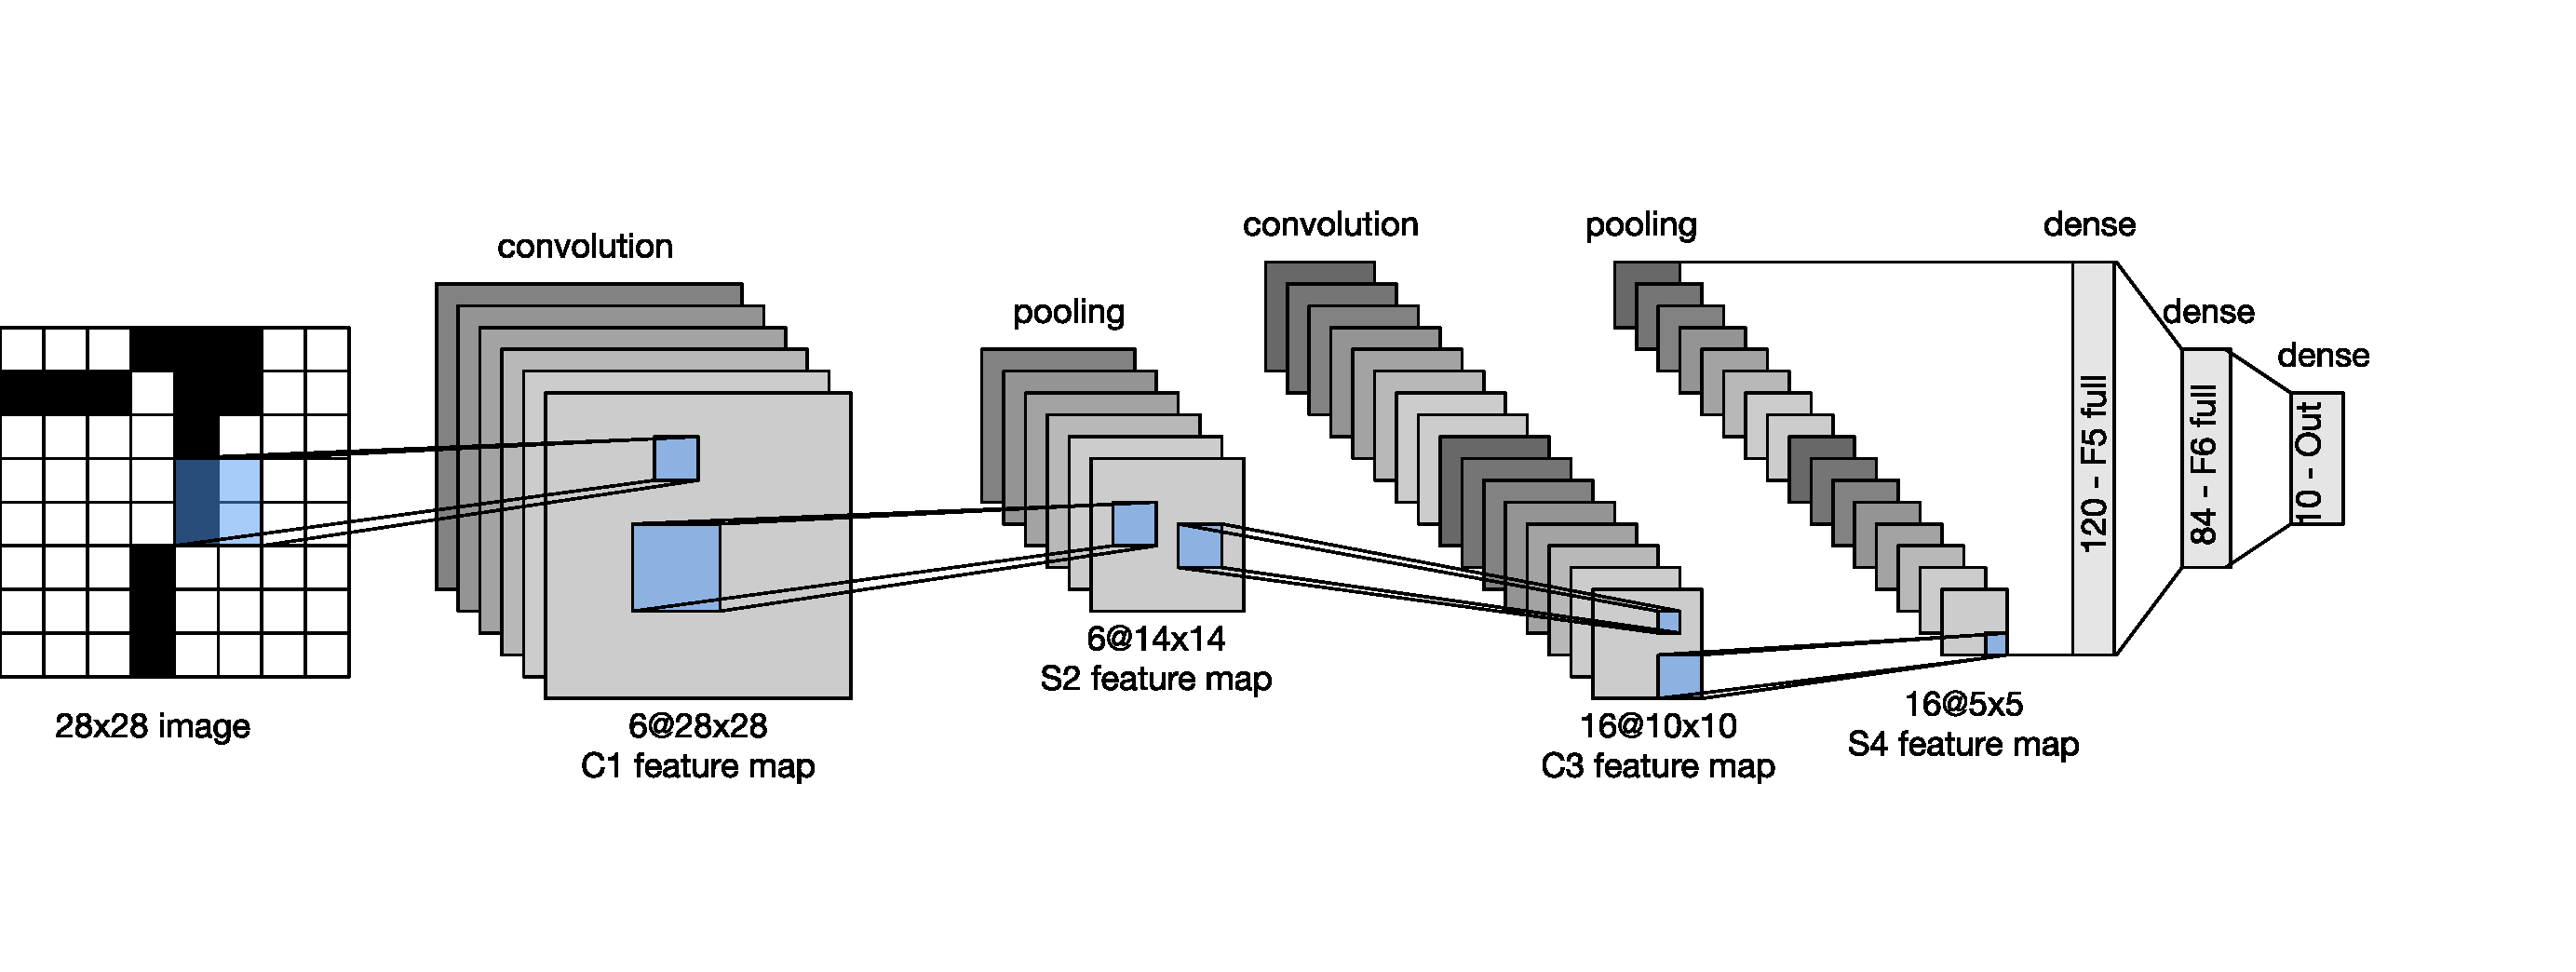
\includegraphics[width=150mm]{CNN}
  \caption[Convolutional Neural Network architecture]{Convolutional Neural Network architecture. Reprinted from \cite{venkatesan_li_2017}.}
  \label{fig:cnn}
\end{figure}

\subsection{Generative models}

In machine learning, there are mainly three types of learning algorithms: supervised learning algorithms, unsupervised learning algorithms, and semi-supervised learning algorithms. The supervised learning algorithms make use of labeled data for its training process. In the last years, this kind of algorithm is presenting significant results in applications like object detection \cite{Liu2019}.

The unsupervised learning algorithms are the ones that do not need a structured dataset and they can find the underlying pattern by itself. One particular type of semi-supervised learning algorithms are the generative models which work in a specific domain data. The generative models are algorithms that are capable of learning the probabilistic data distribution of some datasets, allowing them to generate new samples similar to the ones in that dataset. Two types of generative models are the variational autoencoders (VAE) and the generative adversarial networks (GAN).

\subsubsection{Autoencoders}

In a similar way as the CNNs, the autoencoders are an extension of the deep feedforward network, with the difference that in this case, the goal is to replicate the input in the output. This type of networks are divided in two parts: the encoder that tries to generate a latent space \begin{math}h\end{math} where some features are extracted from the input data \begin{math} h = f(x) \end{math}; and the decoder that takes the latent space generated by the encoder as input and reconstructs the data \begin{math} r = g(h) \end{math}. One of the main applications of this type of neural network is the dimensionality reduction, image compression, image denoising or image generation. The image generation case is covered in more detail in the next section with the variational autoencoders as part of the generative models.

\begin{figure}[htb]
  \centering
  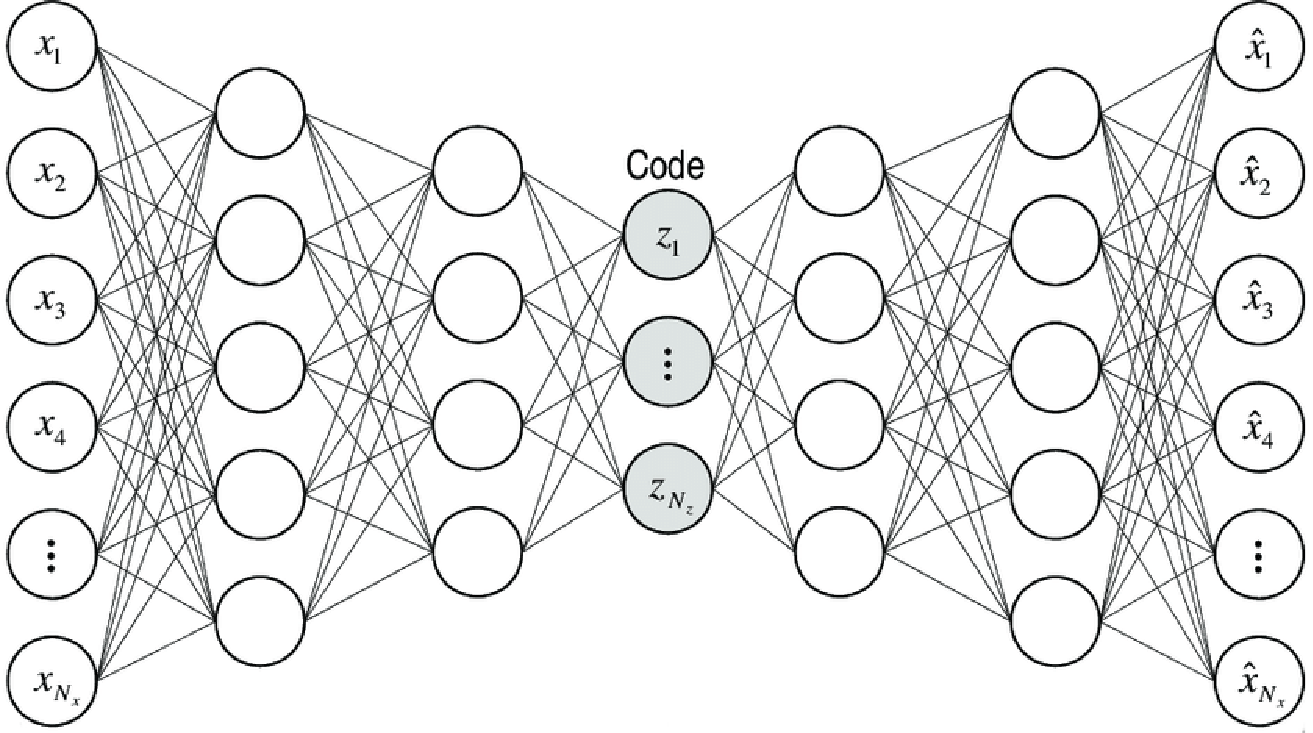
\includegraphics[width=80mm]{autoencoder}
  \caption[Autoencoder architecture]{Autoencoder architecture. Reprinted from \cite{canchumuni_emerick_pacheco_2019}.}
  \label{fig:autoencoder}
\end{figure}

\textit{Variational Autoencoder}

The objective of the variational autoencoders \cite{Kingma2014} is the generation of data samples from a learned latent space. This latent space is obtained from a large dataset. In order to achieve this generation process, these autoencoders must try to learn the probability distribution \begin{math} P(x) \end{math} of the data.

From a probabilistic perspective, the latent variables will be drawn from a prior \begin{math} P(z) \end{math} and the generated data has a likelihood of \begin{math} P(X|z) \end{math} that is conditioned by the latent space. So the goal here is to model the data distribution as follows:

\begin{equation}
 P(X)=\sum_{z} P(X | z) P(z)
\end{equation}

However, this integral is computationally untractable, due to the impossibility of computing all elements in the latent space. To avoid this, VAEs try to infer the distribution \begin{math} P( x ) \end{math} from data using \begin{math}P(z|X)\end{math}. Variational inference approximates the distribution \begin{math}\mathbb{P}(z | X)\end{math}, using a simpler distribution, where a common choice is a Gaussian distribution. Then, with a parametric inference model \begin{math}Q(z|X)\end{math} that maps the input data into the latent space; the difference between the distribution \begin{math}P(z|X)\end{math} and \begin{math}Q(z|X)\end{math} is calculated using the Kullback-Leibler divergence.

\begin{equation}
 \begin{aligned} D_{K L}(Q(z | X) \| P(z | X)) &=\sum_{z} Q(z | X) \log \frac{Q(z | X)}{P(z | X)} \\ &=\mathbb{E}\left[\log \frac{Q(z | X)}{P(z | X)}\right] \\ &=\mathbb{E}[\log Q(z | X)-\log P(z | X)] \end{aligned}
 \label{eq:dkl}
\end{equation}

Using \begin{math}P(z | X)=\frac{P(X | z) P(z)}{P(X)}\end{math}, \ref{eq:dkl} can be rewritten as:

\begin{equation}
 \begin{aligned} D_{K L}(Q(z | X) \| P(z | X)) &=\mathbb{E}\left[\log Q(z | X)-\log \frac{P(X | z) P(z)}{P(X)}\right] \\ &=\mathbb{E}[\log Q(z | X)-\log P(X | z)-\log P(z)+\log P(X)] \end{aligned}
\end{equation}

\begin{math}P(x)\end{math} does not depend on \begin{math}z\end{math}, hence it can be taken out of the expectation:

\begin{equation}
 \begin{aligned} \Longrightarrow \log P(X)-D_{KL}(Q(z | X) \| P(z | X)) &=\mathbb{E}[\log P(X | z)]-\mathbb{E}[\log Q(z | X)-\log P(z)] \\ &=\mathbb{E}[\log P(X | z)]-D_{KL}(Q(z | X) \| P(z)) \end{aligned}
 \label{eq:vae_loss}
\end{equation}

Since the \begin{math}D_{KL}\end{math} is always positive, \ref{eq:vae_loss} can be written as:

\begin{equation}
 \log P(X) \geq \mathbb{E}[\log P(X | z)]-D_{KL}(Q(z | X) \| P(z))
 \label{eq:ineq}
\end{equation}

The first term of the loss function can be seen as the reconstruction error and the second term corresponds to the KL error \cite{Doersch2016}.

\textit{Spatial Variational Autoencoder}

Consist of an improvement of the typical variational autoencoder. Whereas in the classic VAEs the latent space are vectors where their components have a dimension of 1x1, in the spatial VAE the idea is to extend these latent variables to have a higher dimension and, in that way, to be able to capture more spatial features of the input data.

In \cite{Wang2019} a spatial variational autoencoder is proposed, where the latent variables are sampled from a matrix-variable normal (MVN) distribution. The authors claim that this architecture outperforms the original VAEs due to the capture of richer structural and spatial information from data.

\textit{Gaussian-Mixure Variational Autoencoder}

This architecture corresponds to another variant of the VAEs models. In this case, the prior distribution \begin{math}\mathbb{P}(z)\end{math} is a Gaussian-mixture that allows the net to perform unsupervised clustering of the data. This autoencoder, proposed in \cite{Dilokthanakul2016}, has the potential of grouping the data, and each group can represent or share a specific feature of the original data. It has a competitive performance in comparison with the regular VAEs.

\subsubsection{Generative adversarial networks}

The generative adversarial networks (GAN) were proposed by Ian Goodfellow \cite{Goodfellow2014} in 2014. The basic idea behind GANs is in the contest of two models: on one side, there is the generator $G$ that tries to learn the probability distribution of the data and for the other side, a discriminator $D$ that decides if the input data is real or generated by $G$. The goal of the generator is to try to create images as real as possible that provokes the discriminator to make mistakes.  This game is described as the minmax value function in \ref{eq:gan}.

\begin{equation}
 \min _{G} \max _{D} V(D, G)=\mathbb{E}_{x \sim p_{\text {data }}(x)}[\log D(x)]+\mathbb{E}_{z \sim p_{z}(z)}[\log (1-D(G(z)))]
 \label{eq:gan}
\end{equation}

A well trained GAN model is able to reach the Nash equilibrium, where the discriminator has an accuracy of around 0.5, which means that it is not able to discern between fake or real data; and the generator should reach value loss of approximately 0.7.

\begin{figure}[htb]
  \centering
  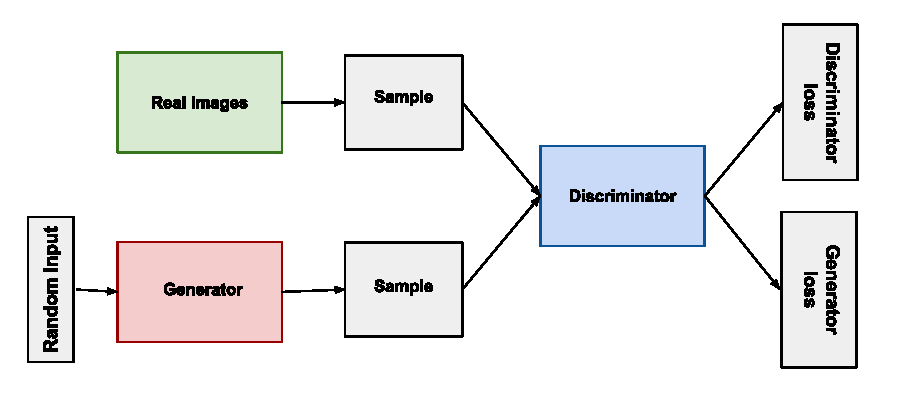
\includegraphics[width=120mm]{gan_diagram}
  \caption[Generative Adversarial Network architecture]{Generative Adversarial Network architecture. Reprinted from \cite{overview_of_gan_structure}.}
  \label{fig:gan}
\end{figure}

One of the challenges that the GANs face is precisely the training process, since depending on the initial conditions the Nash equilibrium is never reached. If the capacity of the model is too small, the model is susceptible to collapse. Another possible scenario is when the learning rate of the model is too aggressive, causing that the net never converges.

\textit{Architectures based on GANs}

In \cite{Pan2019} a series of architectures based on GANs is presented, along with some metrics to evaluate their performance.

\begin{itemize}
 \item \underline{Convolution base GAN}: The original GAN is implemented based on the multi-layer perceptron but it has been proven that CNN are better than the MLP in extracting features to the images. This kind of network is known as Deep Convolutional Generative Adversarial Network (DCGAN).
 \item \underline{Conditional GAN}: Normally, the generator in the GAN receives as input some random noise, which sometimes makes the model prone to collapse. It is for this reason that in the conditional GAN a variable C is introduced as input to the generator and also to the discriminator, with the objective of add some constraints and, therefore, to have more control in the latent space. The type of constraint will depend on the type of data that the GAN is dealing with.
 \item \underline{Autoencoder based GAN}: This type of GAN architecture is presented in \cite{Makhzani2015} where the idea is to make use of an adversarial training to the autoencoder performing variational inference by matching the aggregated posterior latent space of the autoencoder with an arbitrary prior distribution. This allows to overcome one of the main challenges of the autoencoders, when it is not able to correctly learn the data distribution.
\end{itemize}

\subsection{Use of generative models in the anomaly detection}

The generative models discussed so far, find application in the detection of anomalies. The general idea is to train a model capable of learning the data distribution of a regular dataset. In that way, the model should be able to reconstruct o generate a query image as similar as possible and then compare the original with the reconstructed images. If for some reason that is not the case, there is a high probability that the regions that the model was not able to generate, correspond to an anomaly. All the autoencoders described before can be used in this way, as well as the GANs.

For the specific case of the GANs, in \cite{DiMattia2019} different GAN based architectures is presented, with the purpose of anomaly detection:

\subsubsection{AnoGAN}

This GAN is first trained with just regular data and is intended to learn the manifold of the data $x$. Then, with the generator trained, each time that some image has to be evaluated, an iterative process is performed in order to find the latent variables that generate the output \begin{math}G(x)\end{math} most similar to the query image. This iterative process has the disadvantage that is too time-consuming \cite{Schlegl2017}.

\begin{figure}[htb]
  \centering
  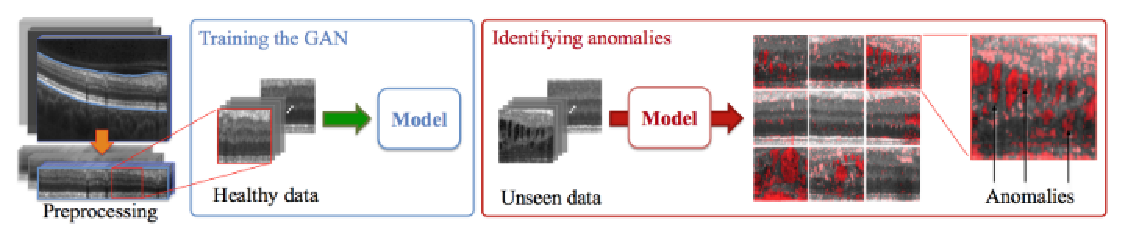
\includegraphics[width=150mm]{anogan}
  \caption[AnoGAN]{AnoGAN traing with healty images first and then reconstruction of unseen images. Reprinted from \cite{Schlegl2017}.}
  \label{fig:anogan}
\end{figure}

\subsubsection{GANomaly}

This architecture is inspired by the AnoGan but tries to overcome the long detection times. In order to do that, it makes use of an encoder that is able to learn the latent space variables that the generator receives during the GAN training. This has the advantage of having a faster GAN training and reduces the times to generate a similar image to the query image. The generator also has an encoder at the end of its structure that helps during training to learn the manifold of the input data $x$.

\begin{figure}[htb]
  \centering
  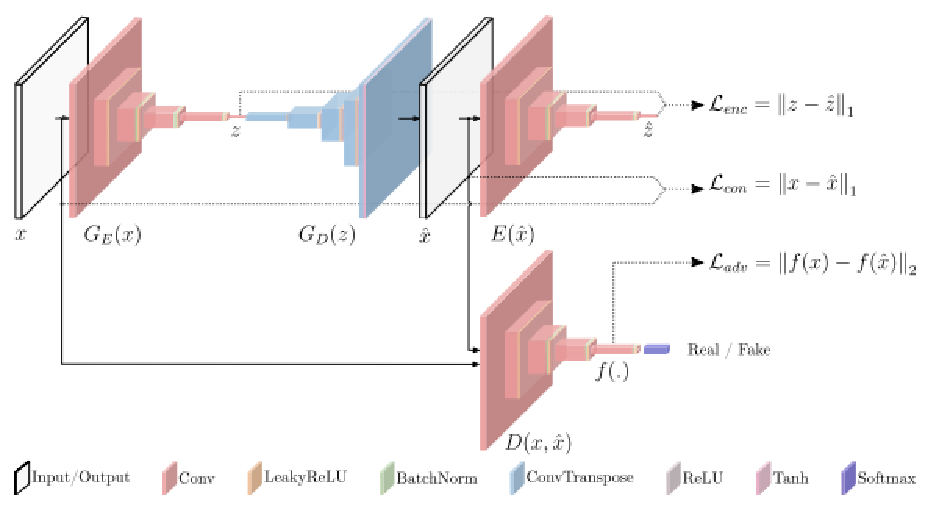
\includegraphics[width=130mm]{ganomaly}
  \caption[GANomaly]{GANomaly architecture and loss functions. Reprinted from \cite{DiMattia2019}.}
  \label{fig:ganomaly}
\end{figure}
